\clearpage
\section{Design and Implementation of \coordtool}
\label{ch:por:sect:coord}
In this section we provide a detailed explanation on various points of the design
and implementation of \coordtool, which adapts applications to run with \tool\
and \gemini\ under \PRCN.

\subsection{Design rationale}

To minimize coordination overhead, in addition to apply the analysis presented 
in Section~\ref{ch:por:sect:identify} for statically extracting a minimal set 
of restrictions, we aim to build an efficient coordination service for enforcing
restrictions at runtime. This is challenging due to the following observation.
We observed that there exist several coordination techniques/protocols that can be used
for enforcing a given restriction, such as Paxos, distributed locking, or escrow techniques. However, depending on the
frequency at runtime in which the system receives operations confined by a restriction, different coordination approaches 
lead to different performance tradeoffs. A challenging question
we need to answer is: how to choose a cheapest protocol for a restriction?

Consider the previously mentioned RUBiS example. In this example,
maintaining the invariant that winners always match highest 
bidders requires a restriction between any pair of {\tt placeBid'}
and {\tt closeAuction'}. The simplest coordination policy would be forcing the two types of shadow operations to pay the same coordination
cost for figuring out the existence of concurrent peers. However, this solution yields a very poor performance due to the imbalanced workload
between the two types of shadow operations, i.e., {\tt placeBid'} is more prevalent than {\tt closeAuction'}. As a result, reducing the latency for 
{\tt placeBid'} while maintaining the corresponding ordering constraint will comprise
a good user experience. 

In summary, we propose to build a specialized coordination service called \coordtool\ offering
coordination policies, each of which presents a tradeoff between the cost of each operation and 
the overall cost. This service allows us to use runtime information about the relative frequency of operations
to select an efficient coordination mechanism for a given restriction that has lowest cost. 

\subsection{Coordination protocols}
\label{ch:por:sect:coordination}
In this part, we present the two coordination techniques that
we currently support in \coordtool\ and concrete
scenarios where these mechanisms are more adequate. We leave to
the future work the implementation of more techniques so that
programmers have more choices for their various tradeoff points. 
The two implemented protocols are namely, {\tt symmetry (Sym)} and {\tt asymmetry (Asym)}.
Given a restriction $r(u, v)$ between two operations $u$ and $v$, the 
{\tt symmetry} protocol requires both $u$ and $v$ to contact each other
for establishing an order between them. Unlike this, an {\tt asymmetry} protocol
provides different treaties for $u$ and $v$ by
only requiring $u$ (or $v$) to inform the counterpart operation in the restriction $v$ (or $u$) 
about its existence, while allowing $v$ (or $u$) to be fast executed without coordination 
if no $u$ (or $v$) operations are running simultaneously. We illustrate the two protocols as follows:

\paragraph{{\tt Sym:}} This protocol requires us to set up a centralized counter service, 
which maintains a counter for every shadow operation, i.e., $c_{u}$ and $c_{v}$,
and serializes reads and writes to these counters. Every such counter represents the total number of the corresponding
operation have been accepted by the underlying system. Additionally, every replica at different
data centers maintains a local copy of the counters, each of which represents the number of the corresponding
operation have been observed by that replica. Initially all local copies as well as the global counters have 
all values set to zero. Whenever an $u$ operation is received by a replica, 
that replica would contact the counter service to increase the
corresponding counter $c_{u}$ and get a fresh copy of the counter maintained
for $v$. Upon receiving the reply from the counter service
that replica can then compare the value of $c_{v}$ with its local copy.
If they are the same, then the replica can execute $u$ without waiting. If the value is greater than
the local copy, the local execution can only take place when all missing $v$ operations have been locally replicated.
The same procedure is also applied to $v$, vice versa. After replicating operations, 
the {\tt cleanUp} is called to bring the local copy of the counters to be up-to-date.
In order to make the counter service fault tolerant, we leverage the Paxos-like state machine replication technique (BFTSmart~\cite{Bessani2014SMR}) to 
replicate the service state in a few geo-locations.


\paragraph{{\tt Asym:}} Unlike the above centralized solution, the core of the asymmetry protocol
implements distributed barrier and operates via a decentralized manner as follows. Assume, for
simplicity that $u$ is the barrier. In this case whenever
a replica $r$ receives an operation $u$ it would have to enter the barrier,
and contact all other replicas to request this. This requires all
replicas in the system to stop processing $v$ operations.
After all replicas acknowledge the entrance of $r$ in the barrier for $u$, $r$ can execute the operation, and then notify all replicas 
that it has left the barrier (while at the same time propagating the effects
of the operation $u$ it has just executed).
Such a coordination strategy might incur
in a high overhead; however, it might be interesting when one of
the two operations in the restriction is rarely submitted to the system.
For instance, in the auction example, {\tt closeAuction'} is
a candidate for being used as barrier, since 
{\tt placeBid'} dominates the operation space.




\subsection{Interfaces}
\begin{figure}[t!]
\centering
\pseudocodeinput[breaklines=true,mathescape=true]{pseudocode/por/olisipoInterface.txt}
\caption{Olisipo library interface}
\label{fig:por:olisipinterface}
\end{figure}
In order to accommodate different protocols in \coordtool, we design a set of generic interfaces
for understanding the programmer specified restrictions and invoking proper protocols for ensuring
decided restrictions. Figure~\ref{fig:por:olisipinterface} shows the interfaces that library exposes to programmers. 
{\tt getPermissions} takes the transaction id and the operation name as input, and produces a permission as return.
{\tt waitForBeingExecuted} executes a loop and only exits if the returned permission is locally satisfied. {\tt cleanUp}
function removes all used resources and data structures for executing the corresponding shadow operation. The lifecycle of
every produced shadow operation will be as follows: {\tt getPermission} $\rightarrow$ {\tt waitForBeingExecuted} $\rightarrow$ {\tt cleanUp}.

\subsection{Architecture}
\label{sec:tool}
\begin{figure}[t!]
\centering
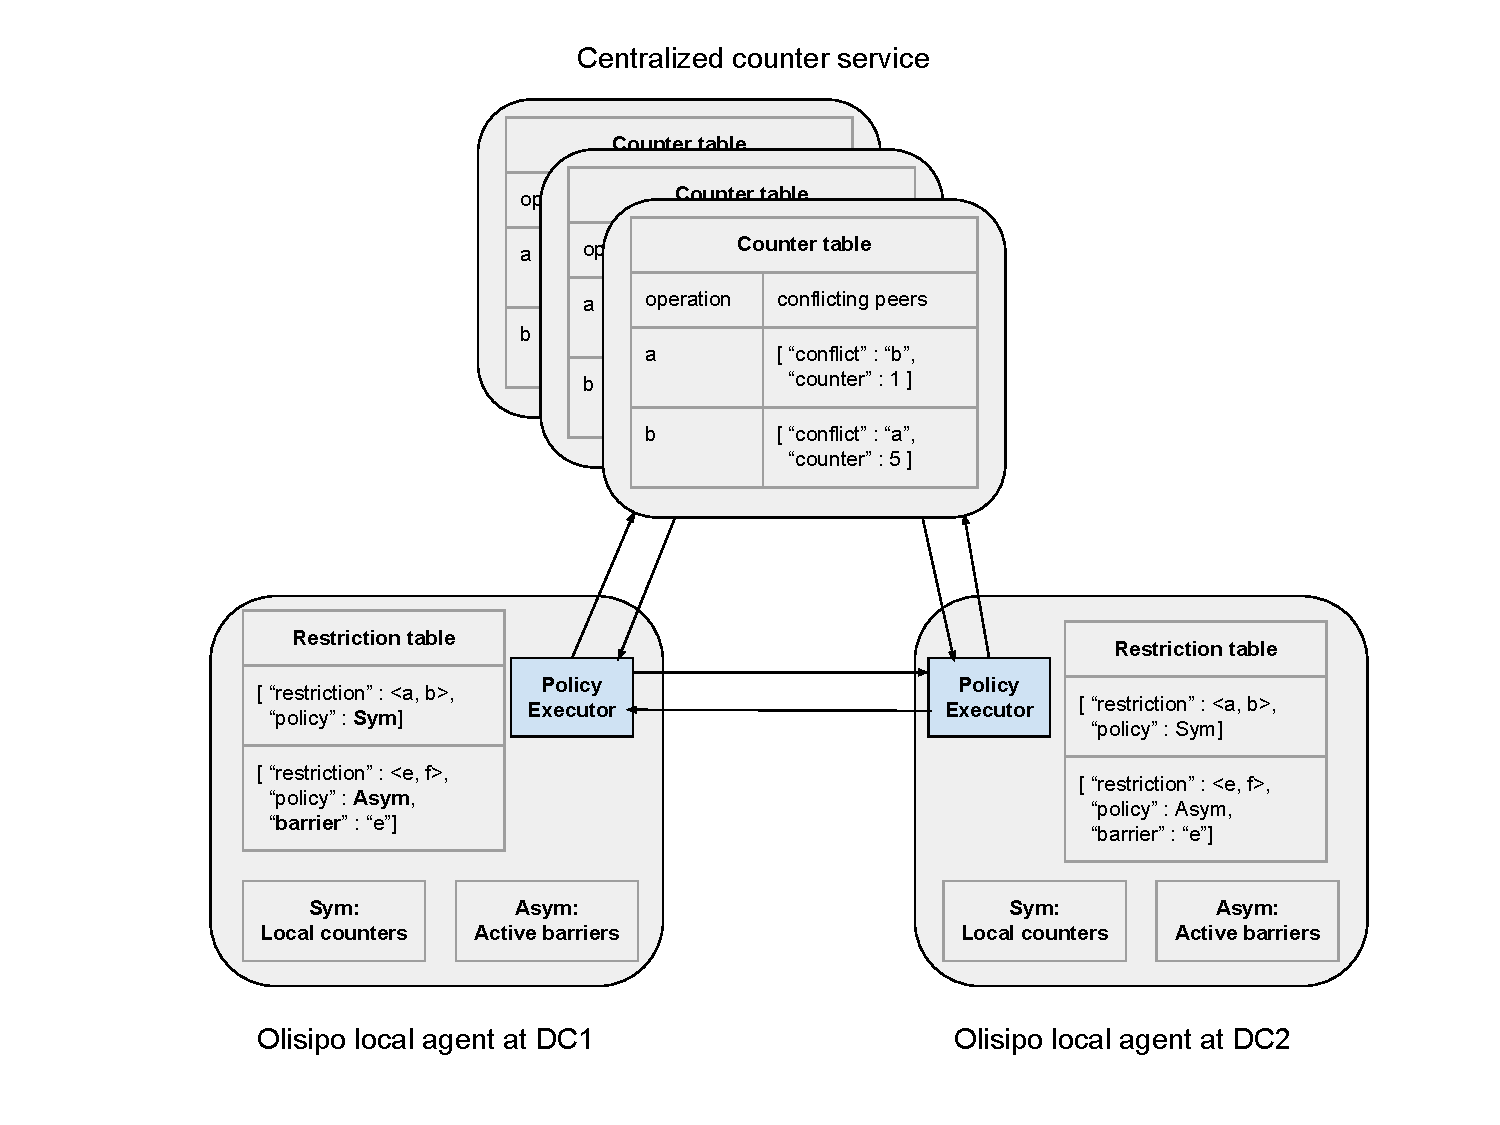
\includegraphics[width=\columnwidth]{./figures/por/tool_support.pdf}
\caption{\coordtool\ architecture}
\label{fig:tooldesign}
\end{figure}

All design choices and details presented above lead to the high level system architecture 
depicted in Figure~\ref{fig:tooldesign}. The \coordtool\ architecture consists of a replicated counter service across data centers and a local agent deployed
in every data center. While the counter service is required by executing the {\tt Sym} protocol
for keeping track of the number of different operations that have been accepted by the system.
the local agent is responsible for placing coordination only when the corresponding
operation is confined by restrictions. Every local agent keeps a restriction table, which defines
all identified restrictions between pair of operations and the corresponding coordination policy.
In addition, every agent also stores some meta data required for different protocols. With regard
to the {\tt Sym} protocol, it maintains a local copy of the replicated counter service, which is used
for learning if the local counters lag behind the global counters, which means
the corresponding data centers have to wait until all missing operations have been locally
incorporated. For the {\tt Asym} protocol, every agent maintains a list of active barriers, which
are used for locally deciding if the counterpart operations of such barriers can proceed or must wait.

\begin{figure}[t!]
\centering
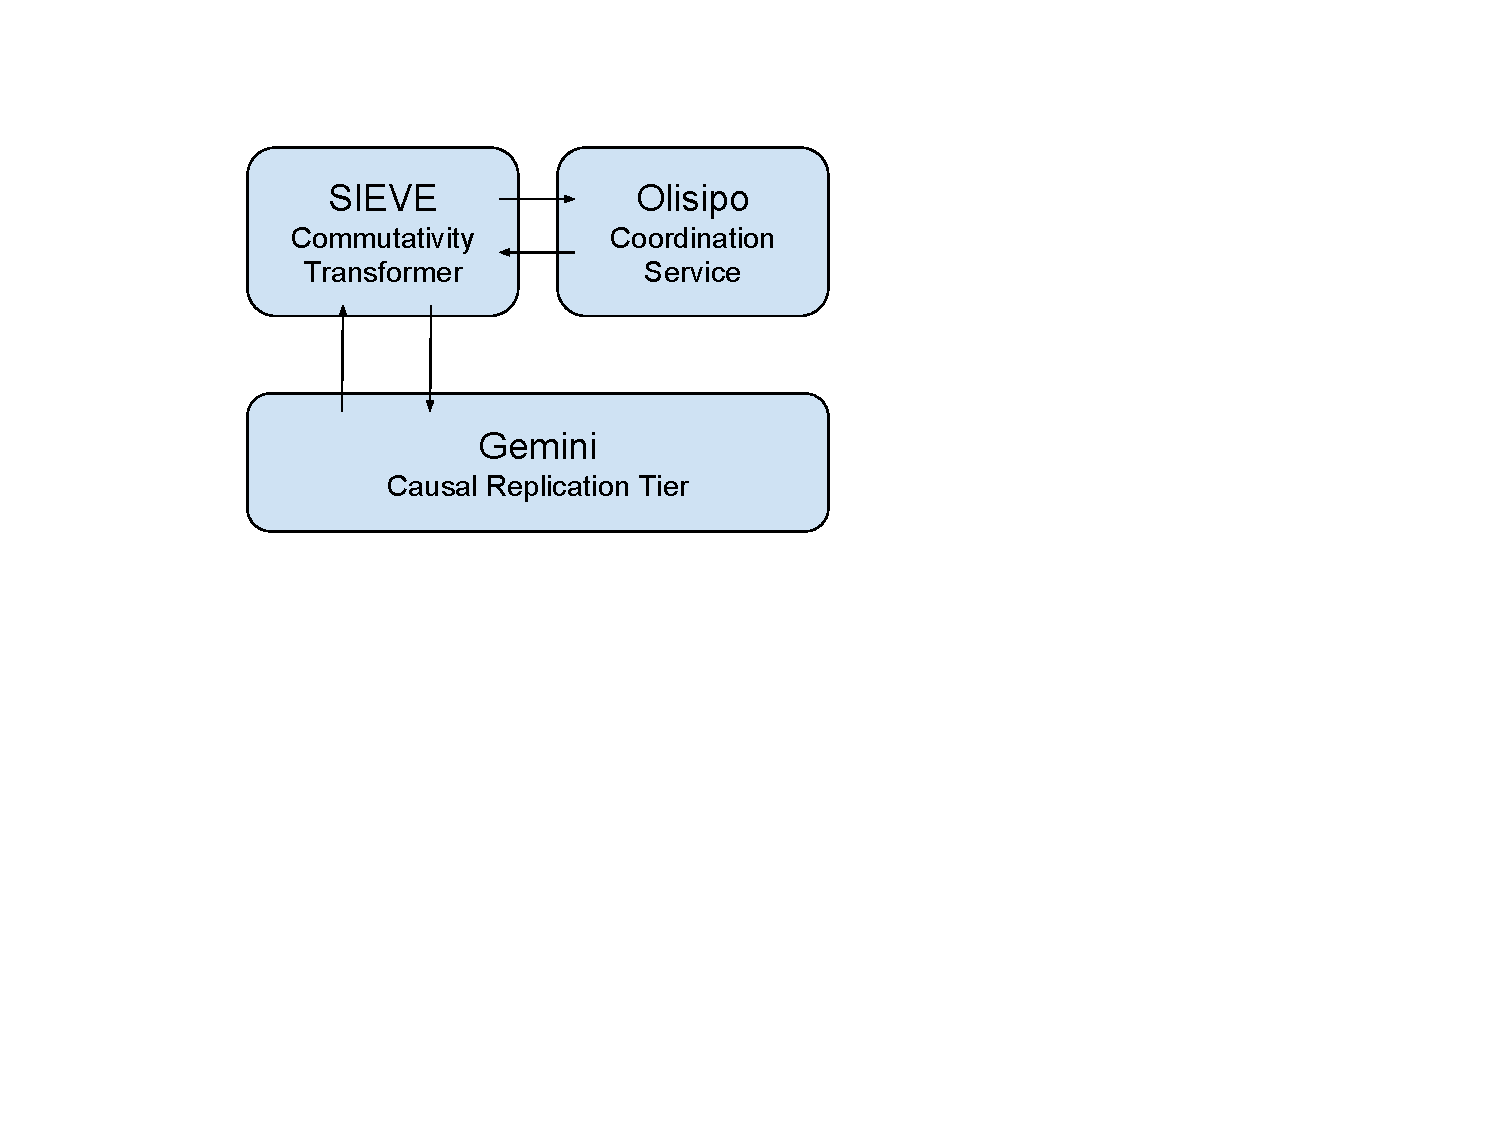
\includegraphics[width=0.76\columnwidth]{./figures/por/tool_intergated.pdf}
\caption{\coordtool\ connected with \tool\ and \gemini}
\label{fig:toolwithenvironment}
\end{figure}

\subsection{Implementation}
We implemented \coordtool\ using Java ($2.8k$ lines of code)~\footnote{The lines of code is
measured by {\tt cloc}~\cite{codecounter}.}, and used BFTSmart~\cite{bftsmartcode} for replicating
the state of the centralized counter service, MySQL as the backend storage, and Netty
as the communication library~\cite{Netty}. As shown in Figure~\ref{fig:toolwithenvironment},
we integrated \coordtool\ with \gemini\ and \tool\ so
that \gemini\ serves as the underlying causally consistent replication tier while \tool\ is used to
produce commutative shadow operations at runtime. 

\noindent\paragraph{Workflow:} A user issues her request to an application server locating at a nearby
data center, which runs a \tool\ library introduced in Chapter~\ref{chapter:sieve} and
a local agent shown in Figure~\ref{fig:tooldesign}. \tool\ intercepts the communication between
the app server and the backend MySQL database and executes the corresponding generator operation.
When the execution ends, \tool\ produces a commutative shadow operation that accumulates side effects
of that request, and then asks the \coordtool\ local agent for placing coordination if needed before committing and replicating
that shadow operation. To do so, \coordtool\ agent lookups into the restriction table
if that operation is confined by any restriction. If so, then the {\tt policy executor} residing
\coordtool\ orders that operation with respect to all its conflicting operations that are running concurrently
at other data centers. This is achieved by invoking a sequence of functions 
presented in Figure~\ref{fig:por:olisipinterface} associated with different protocols 
according to the lookup result, i.e., which protocols to be used. 
At the end, when conflicting operations are accordingly serialized, \tool\ sends these
operations to \gemini\ for replicating them across all data centers while respecting the established order. 
The sourcecode of \coordtool\ is available at ~\cite{olisipocode}.

